\chapter{Rolling Rank IC — Comparativo entre Modelos}
\label{ap:rolling_ic}

\begin{figure}[htbp]
    \centering
    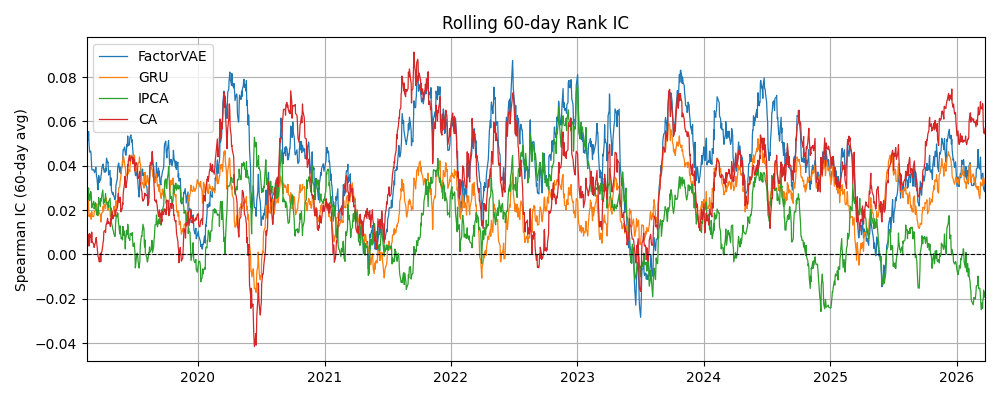
\includegraphics[width=\textwidth]{figuras/RIC_rolling_rank_ic.png}
    \caption{Rank IC médio móvel de 60 dias — FactorVAE vs.\ benchmarks (2019--2026).}
    \label{fig:rolling_rank_ic}
\end{figure}

Ao longo de todo o período de teste, o FactorVAE mantém Rank IC predominantemente positivo e superior à maioria dos concorrentes, com picos acima de 0{,}08 em 2021--2022 e em 2023. O GRU apresenta desempenho positivo, porém mais moderado e próximo à média dos benchmarks. O IPCA exibe maior variabilidade, com episódios prolongados de IC negativo --- notavelmente em meados de 2023 e no final de 2025. O CA acompanha o FactorVAE em vários subperíodos, mas com amplitude ligeiramente menor. A vantagem do FactorVAE é mais pronunciada em janelas de maior volatilidade, o que sugere que a estrutura variacional captura melhor a dinâmica fatorial em regimes de estresse.